\documentclass[twoside]{wiss}

%\usepackage{ascmac}
\usepackage[hiragino-pro]{luatexja-preset}

\usepackage{graphicx}
% \usepackage{here} % [H]とするとその場所に配置されるらしい

\usepackage{balance}    %% 最後のページの高さを揃えるために追加  (2012/9/27:watanabe, Igarashi)

\journalhead{Babascript: }

\begin{document}

\title{Babascript: }
\etitle{Babascript: }

\author{匿名で査読を行うため著者名なし
  \affil{匿名で査読を行うため所属名なし}}

\maketitle

\begin{abstract}
  本論文では、Babascriptを提案する

\end{abstract}

% \input{.tmp/introduction.tex}
% \input{.tmp/babascript.tex}
% \input{.tmp/system.tex}
% \input{.tmp/application.tex}
% \input{.tmp/discussion.tex}
% \input{.tmp/prework.tex}
% \input{.tmp/conclusion.tex}
\begin{abstract}

何かしらの処理を実行するとき、コンピュータが得意なことはコンピュータに、人は人にしかできないことや人がやるべきことに集中すべきだ。何かしらの処理を実行するとき、コンピュータが得意なことはコンピュータに、人は人にしかできないことや人がやるべきことに集中すべきだ。何かしらの処理を実行するとき、コンピュータが得意なことはコンピュータに、人は人にしかできないことや人がやるべきことに集中すべきだ。何かしらの処理を実行するとき、コンピュータが得意なことはコンピュータに、人は人にしかできないことや人がやるべきことに集中すべきだ。何かしらの処理を実行するとき、コンピュータが得意なことはコンピュータに、人は人にしかできないことや人がやるべきことに集中すべきだ。何かしらの処理を実行するとき、コンピュータが得意なことはコンピュータに、人は人にしかできないことや人がやるべきことに集中すべきだ。

\end{abstract}

\maketitle

\section{はじめに}\label{ux306fux3058ux3081ux306b}

人にはAPIがない。
APIがないということは、既存のプログラムから人に対して何か要求したり、命令することは困難である。

だが、実世界の要素はAPIを持つようになっている。
ユビキタスコンピューティングや実世界志向インタフェース等の研究によって、あらゆるモノにコンピュータが組み込まれ、プログラムによって操作されるようになる日は近い。
また、既に実商品として、プログラマブルな電球などが販売されており、既に生活の中にAPIを持った要素を組み込んでいくことが出来る状況にある。

世界がプログラムで記述できるようになっていく中で、人への命令をプログラムで記述できるような取り組みは少なく、クラウドソーシング等の分野における研究が目立っている。
また、その用途も限定的なものが多い。
人への行動命令を含んだプログラムが記述できるようになれば、生活や社会といったような、人を処理の中に含んだプログラムが記述可能となり、あらゆることがプログラムによる自動化の恩恵を受けられる。

人がシステムを使うことを主眼にするのではなく、人がシステムを使うことを含んだ全体を記述できるようになれば、あらゆることが自動化可能になるのではないか

コンピュータが得意なことはコンピュータが、人が得意なことは人が処理を実行していく相補的な関係が望ましい

そこで本論文では、人に対してプログラム上から処理命令を送り、その処理の結果を返り値として受け取ることを実現する一連のシステム
Babascript を提案する。

\section{Babascript
プログラミング環境}\label{babascript-ux30d7ux30edux30b0ux30e9ux30dfux30f3ux30b0ux74b0ux5883}

Babascript環境では関数呼び出しによって人に命令を送る仕組みによって、プログラム内での人への処理命令を実現する。
通常のプログラムでは、関数に引数を与え実行することで、処理結果を返り値として得ることができる。
Babascriptでは、同様に関数呼び出しし、処理を人に実行させ、返り値を処理結果として返す。
つまり、同じ関数呼び出しだが、その実行主体を人間にすることによって、プログラム内における人力処理の組み込みを実現する。

このような仕組みを実現するために、人への命令構文を持ったDSL Babascript
と、命令に対して返り値を返すためのクライアントライブラリ Babascript
Client、クライアントライブラリを組み込んだWebアプリケーションを実装した、
また、プラグイン機構によってその機能を拡張可能にした。

\begin{figure}[h]
  \centering
  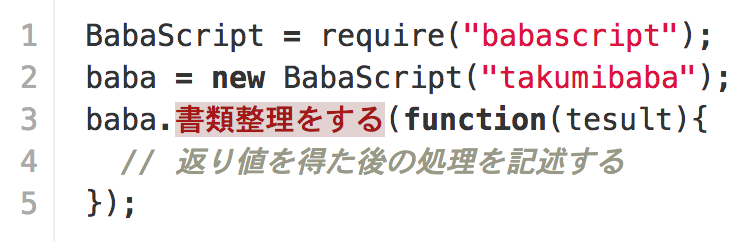
\includegraphics[width=220px]{./images/script_01.png}
  \caption{babascriptプログラムの基本命令文}
  \label{script_01}
\end{figure}

\subsection{BabaScript}\label{babascript}

Babascriptは、関数呼び出しによって人に対して処理命令を送れるオブジェクト(以下、人オブジェクト)を宣言可能にするDSLだ。
人オブジェクトにおいて定義されていない全てのメソッドが人への命令として解釈される。
また、命令に対して人からの返り値を得ると、実行メソッドの引数で指定したコールバック関数を実行する。

\subsubsection{人オブジェクトの宣言と処理命令構文}\label{ux4ebaux30aaux30d6ux30b8ux30a7ux30afux30c8ux306eux5ba3ux8a00ux3068ux51e6ux7406ux547dux4ee4ux69cbux6587}

図\ref{script_01}のようなプログラムによって、人への処理命令を送ることができる。
人への処理命令構文は、実行されるとメソッド名と引数を元にしたjsonオブジェクトへと変換され、このjsonオブジェクトが処理命令のデータとしてクライアントライブラリに配信される。

人オブジェクトは宣言時にIDを指定することによって、誰に対して処理命令を配信するかを決定する。
実行された処理命令は、指定したIDを監視するクライアントライブラリにのみ配信される。
この際、指定したIDを監視するクライアントが複数人、つまり、グループを形成していた場合、人への命令構文を実行時に他のタスクを実行していないクライアントへと順番にタスクが配信される。

人への処理命令構文の第一引数には基本的な処理情報に加えてクライアント側に送信するオプション情報を指定する。
第二引数には、人から処理命令に対する返り値が得られた際に実行するコールバック関数を指定する。
コールバック関数実行時には、その引数に返り値と関連した情報を格納したオブジェクトが与えられる。

オブジェクトに定義されていない全ての関数は人への処理命令構文として解釈される。
この機能はmethodmissingという、定義されていないメソッドが実行された際にその処理を記述しておく仕組みによって実現する。

\subsubsection{オプション情報の付加}\label{ux30aaux30d7ux30b7ux30e7ux30f3ux60c5ux5831ux306eux4ed8ux52a0}

人への処理命令構文の第一引数に与えるオプション情報には、返り値の型指定などの情報が考えられる。
返り値としてあらゆる型を想定したプログラムを記述することは難しい。
例えばBoolean型で返してほしい、といった時には図2のようなプログラムが考えられる。

\begin{verbatim}
baba.ほげふが {format: 'boolean'}, (task) ->
    console.log task
\end{verbatim}

他にも、指定したリストの中から値を選択してほしい、といった命令の場合は、そのリストをオプション情報として付加することが考えられる。

特別なオプション情報として、broadcastオプションが存在する。
broadcast機能は、指定したIDを監視する全てのクライアントへとタスクを配信し、指定した数の返り値を得られると処理を終了し、コールバック関数を実行するといったものだ。

\subsection{BabasciriptClient}\label{babasciriptclient}

\subsubsection{ライブラリ}\label{ux30e9ux30a4ux30d6ux30e9ux30ea}

Babascript
Clientは、Babascriptからの命令受信と処理結果の送信機能を実現するクライアントライブラリだ。
命令受信のイベントに対してコールバック関数を指定することで、処理命令を受け取ることができる。
基本的な利用方法は、図\ref{client}に示す。

\begin{figure}[h]
  \centering
  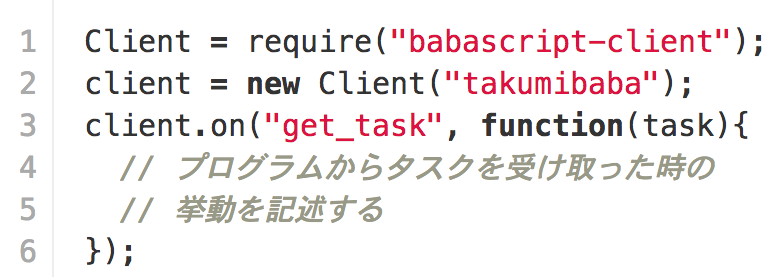
\includegraphics[width=220px]{./images/client.png}
  \caption{クライアントライブラリの基本機能 }
  \label{client}
\end{figure}

クライアントオブジェクトの宣言時、IDを指定することによって、IDに対して処理命令が発行された際にタスクを受信することができる。
また、クライアントオブジェクトが持つ ``returnValue''
メソッドを利用することで、返り値を命令発行元に返すことができる。

クライアントライブラリは、UIと完全に分離した実装となっており、かつ利用方もシンプルだ。
下記のWebアプリケーションだけでなく、新規/既存問わず、様々なアプリケーションに組み込むことができる。

\subsubsection{Webアプリケーション}\label{webux30a2ux30d7ux30eaux30b1ux30fcux30b7ux30e7ux30f3}

BabascriptClientが得たタスクをユーザに提示するためのインタフェースとして、Webアプリケーションを実装した。
タスク情報において型指定をすることによって、ユーザに提示するUIを変化させ、型に合った返り値を選択できるようにしている。
例えば、Boolean型を指定していた場合、ユーザには true ボタンと false
ボタンが提示され、どちらかを押すと、その結果が返り値としてプログラムに返される。
また、String型を指定すれば、文字列の入力フォームとSubmitボタンが表示される。
スマートフォンに最適化したWebアプリケーションとして実装しており、様々な場面において利用可能であり、実世界におけるタスクを処理しながらでも十分に利用可能であると言える。
Webアプリケーションは、図\ref{webapp-interface}のようなインタフェースを持つ。

\begin{figure}[h]
  \centering
  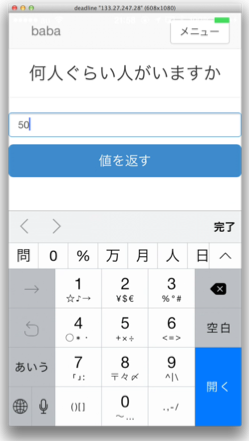
\includegraphics[width=120px]{./images/interface.png}
  \caption{Webアプリのインタフェース}
  \label{webapp-interface}
\end{figure}

\subsection{Plugin}\label{plugin}

Babascript及びBabascript
Clientに組み込むことのできるプラグイン機構を実装した。
Babascript及びBabascriptClientが発行するイベントとデータを受け取り、その都度処理を実行させることができる。
現在、以下のようなイベントが存在する

\begin{itemize}
\itemsep1pt\parskip0pt\parsep0pt
\item
  init(プラグイン読み込み時)
\item
  connect(ネットワーク接続時)
\item
  send(タスクの送信時)
\item
  receive(タスクの受信時)
\end{itemize}

具体的には、以下にょうなプログラムによってプラグインを読み込むことができる

\begin{verbatim}
baba = new Babascript("baba")
baba.use(new Logger())
\end{verbatim}

具体的には、以下のようなプラグインの実装が挙げられる。

\begin{itemize}
\itemsep1pt\parskip0pt\parsep0pt
\item
  ログコレクター
\item
  データ同期
\item
  ユーザ管理
\end{itemize}

\subsection{通信と分散処理}\label{ux901aux4fe1ux3068ux5206ux6563ux51e6ux7406}

scriptとclientのタスク送受信と分散配信のために、node-linda\cite{linda}を利用した。
Websocketによる通信が行われ、リアルタイムにタスクの送受信が行われている。
script,
client共に、このnode-lindaに接続するためのライブラリを組み込んでいる。

scriptは、プログラム実行時にnode-lindaサーバに接続し、人への命令構文を実行するごとに、タスクをnode-lindaサーバに書き込む。
書き込み終了後、そのタスクと同じIDを持った返り値タスクが書き込まれるまで、node-lindaサーバの監視を行う。

clientは、プログラム起動中は常にnode-lindaサーバに接続し、指定されたIDを監視する。

\subsection{処理の流れ}\label{ux51e6ux7406ux306eux6d41ux308c}

Babascript環境は、以下のようなフローで一回の人への命令構文が実行される。

\begin{enumerate}
\def\labelenumi{\arabic{enumi}.}
\itemsep1pt\parskip0pt\parsep0pt
\item
  人への命令構文を実行する
\item
  命令構文に応じたタスクが生成される
\item
  タスクがNode-Lindaサーバを経由してクライアントへと配信される
\item
  タスクを受け取ったクライアントがユーザに処理を促す
\item
  タスク実行者が、処理結果を入力する
\item
  処理結果を元に返り値データが生成される
\item
  Node-Lindaサーバを経由して実行元プログラムに返り値が送信される
\item
  指定されたコールバック関数が実行され、処理が続く
\end{enumerate}

\subsection{実装}\label{ux5b9fux88c5}

上記システムは全てJavascriptで実装した。 Babascript
はNode.js上で動作し、 Babascript
ClientはNode.jsとWebブラウザ上で動作する。
全体図は図\ref{system}のとおりだ。

\begin{figure}[h]
  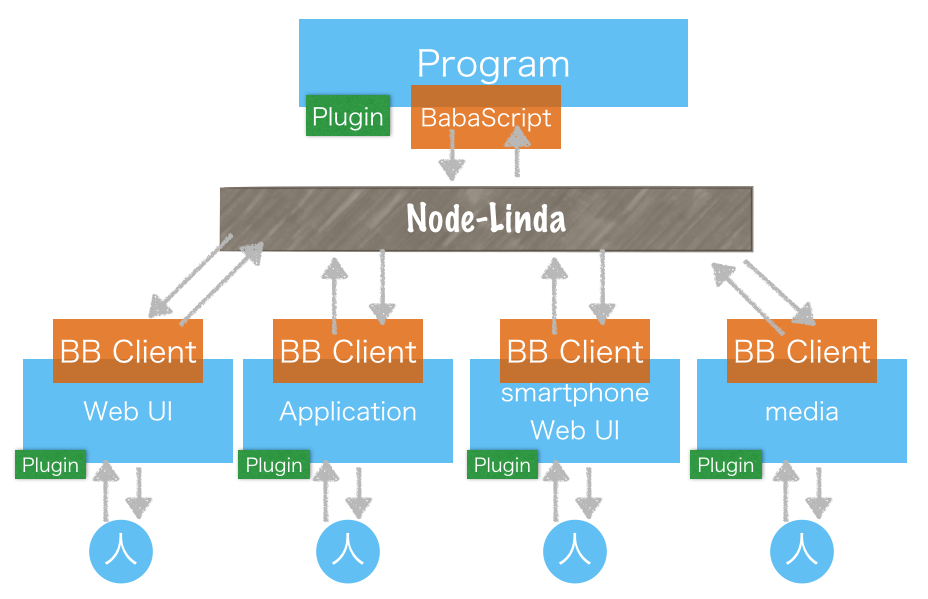
\includegraphics[width=220px]{./images/system.png}
  \caption{システム全体図}  
  \label{system}
\end{figure}

\subsubsection{タスク情報の構成}\label{ux30bfux30b9ux30afux60c5ux5831ux306eux69cbux6210}

人への処理命令構文は実行によってタスク情報を生成する。
このタスク情報は、図\ref{task}のようなjsonオブジェクトとなる。

\begin{figure}[h]
  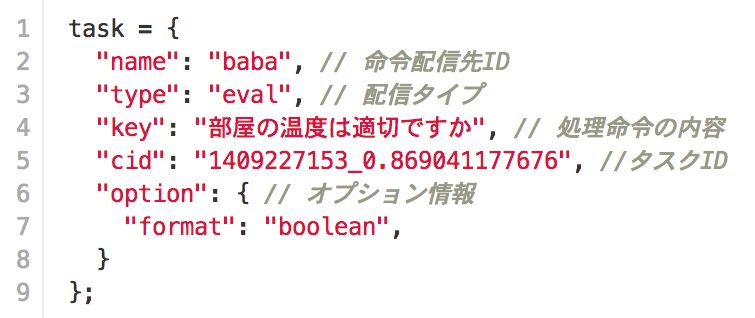
\includegraphics[width=230px]{./images/task.png}
  \caption{タスクのJSONオブジェクト}  
  \label{task}
\end{figure}

\subsubsection{実行結果の待ち方}\label{ux5b9fux884cux7d50ux679cux306eux5f85ux3061ux65b9}

人への命令構文に対する返り値が、適切に返り値として戻されるようにするために、命令ごとにユニークなIDを生成している。
ユニークIDは、人への命令構文実行時のUNIX time
と、ランダムな数値を結合した文字列である。
図\ref{task}におけるjsonオブジェクトの'cid'の項目に示されているものだ。
このユニークIDを伴った返り値が戻ってくるか、指定したタイムアウト時間に到達するか、タスクキャンセルが発生するまで、

\section{応用例}\label{ux5fdcux7528ux4f8b}

以下のような応用が考えられる。

\subsection{仕事や役割をプログラミングする}\label{ux4ed5ux4e8bux3084ux5f79ux5272ux3092ux30d7ux30edux30b0ux30e9ux30dfux30f3ux30b0ux3059ux308b}

人の行動をプログラムとして記述可能になることで、人の仕事や役割がプログラム化・実行可能にするといった応用が考えられる。
仕事や役割はマニュアルやドキュメントという形で言語化されていることが多い。
言語化されているということは、BabaScript
環境を用いることでプログラムとして記述可能である。

プログラム化し、実行可能になれば、人はプログラムからの命令に従うだけで、記述されている内容を実行可能になる。
ただ命令に従うだけなので、経験・引き継ぎは必要なく、人の代替が容易となる。
また、全ての仕事はプログラムから管理されるため、人の運用効率の数値化や進捗の管理などが可能となる。

プログラム化によって、作業をより適切な単位に分割し、逐次的に人に実行させられるようになる。
複雑な作業をしている際、次に何をすれば良いのかといった情報がわからなくなるこ
とがあるが、これは、作業内容を覚えきれていなかったり、忘れてしまうといったことが原因で起こる。
本提案のような仕組みを利用することによって、すべきことの記憶はコンピュータが担うことになる。
人はその時すべきことをプログラムからの命令通りに動作するだけで良い。
コンピュータが判断可能な部分に関しては全てコンピュータに委ねることができるため、人への負担を減らすことができる。

\subsection{実世界をテストする}\label{ux5b9fux4e16ux754cux3092ux30c6ux30b9ux30c8ux3059ux308b}

人をセンサーやアクチュエータとして利用することで、現在一般的に使われているセンサーやアクチュエータでは実現困難な実世界プログラミングが可能となる。
現在のセンサー技術では、その場の雰囲気を数値化・文字列化するなどのコンテキスト情報の分析は困難である。
また、アクチュエータも単一の動きに特化したものが多く、複雑な動きを実現することは難しい。
しかし、人をプログラム上でセンサーやアクチュエータとして利用できれば、既存のセンサーやアクチュエータでは難しい挙動も実現可能である。
BabaScript
環境でならば、プログラム上で人はセンサーやアクチュエータと類似の挙動をすることができる。

また、人とセンサ・アクチュエータを状況に応じて使い分けるといったことも可能となる。
コンテキスト情報を扱いそうなら人を利用し、温度などの数値を取得するだけならばセンサーを利用する、といった使い分けができる。
センサー・アクチュエータがその場に存在するならばセンサー・アクチュエータを動作させるが、ない場合は人に命令する、といったことも実現可能である。

\section{考察}\label{ux8003ux5bdf}

Babascript環境について、以下のように考察する。

\subsection{処理単位としての人}\label{ux51e6ux7406ux5358ux4f4dux3068ux3057ux3066ux306eux4eba}

本研究では、人はコンピュータ等と同じ、処理を命令され実行するノードとなる。
こういった事に対し、心理的な不安等を覚える人が存在するということが考えられる。
しかし、本研究においては、この仕様はやることを出来るだけコンピュータなどに実行させ、人は人にしかできないことや人がやるべきことに集中できるような環境を実現するためのものである。
単純な数値による条件判断などを出来るだけ人間以外の要素に実行させ、人はやるべきことのみを提示され、実行していくということは、全体の処理をうまく処理するという意味において良いことであると考えられる。

\subsection{タスク実行の遅延と実行保障性}\label{ux30bfux30b9ux30afux5b9fux884cux306eux9045ux5ef6ux3068ux5b9fux884cux4fddux969cux6027}

Babascriptによってタスク実行を依頼しても、人がすぐにタスクを実行し値を返すことを完全に保証することはできない。
タスク受信端末を見ていない、受信しても実行できないといった状況の場合、すぐに値を返すことはできない。
こういった際、Babascriptによる処理がボトルネックとなる可能性がある。

また、労働関係にあるなど、タスク実行に強制力がある場合は、タスク実行が確実に行われると考えられるが、強制力がない場合はそもそもタスク受信を無視するといったことも考えられる。
タスク実行に強制力がない場合は、金銭などのインセンティブを与えるといった手段によって、実行保障性を確保するといったことが考えられる。

\subsection{例外処理}\label{ux4f8bux5916ux51e6ux7406}

Babascript環境において、命令文と現実との乖離によって適切な返り値を選択・記述ができなくなるといった可能性がある。
これは、現実が刻々と変化していることなどから、完全に避ける事の出来ない問題であると考える。
この際、無理やり値を返すといった処理をしてしまうと、本来の状態とは違った判断がなされてしまう危険性がある。
命令文とは明らかに現実が異なっている場合などは、タスク実行者のほうで例外としてプログラムに通知出来るような仕組みによって、
問題の解決へと繋げたい。

\subsection{命令内容の粒度}\label{ux547dux4ee4ux5185ux5bb9ux306eux7c92ux5ea6}

Babascriptでは、タスクの文面の記述には制限がないため、自由となっている。
この文面は、適切な抽象度の文面に設計しなくてはならない。
抽象度が高すぎる命令は、あいまいな表記となり、タスク実行者にとって理解しづらい文面となり得る。
その結果、想定外の処理が実行され、意図しない結果を招く恐れがある。
抽象度が低すぎる命令は、全体の処理内容にもよるが、プログラム自体が冗長となり得る。
プログラムとタスク実行者の間のやりとりが増え、通信や待機時間などがボトルネックとなる可能性がある。
また、タスク実行者にとっても、やりとりが増えることで負担増になると考えられる。

\subsection{複数命令の同時実行}\label{ux8907ux6570ux547dux4ee4ux306eux540cux6642ux5b9fux884c}

複数のプログラムから同時に一人のタスク実行者へとタスクが配信される可能性がある。
この際、異なるコンテキストにある命令が交互に配信され、タスク実行に大きな障害をもたらす可能性がある。
例えば、料理プログラムと掃除プログラムが同時に実行された場合、鍋で煮ている途中で「洗剤を投入しろ」などといった命令が配信されることが考えられる。

この問題は、全てのBabascriptプログラム中において、一人のタスク実行者は一つのプログラムからのみ、連続してタスクを受信できるような仕組みを用意することによって、解決可能であると考えられる。
また、応用アプリケーションでの実装になるが、コンテキストを明示し、どの処理系におけるタスクなのかをタスク実行者に示すといった手段によっても解決可能である。

\section{関連研究}\label{ux95a2ux9023ux7814ux7a76}

計算機では処理が難しいようなタスクを解決するために、人を計算資源として利用する手法はヒューマンコンピュテーション\cite{HumanComputation}と呼ばれ、様々な研究が行われている。
インターネットを介して不特定多数の群衆にタスクを実行させるクラウドソーシングと組み合わせた研究事例も多く存在する。
クラウドソーシングのプラットフォームとしては、Amazon Mechanical
Turk\cite{mechanicalturk}が存在する。 Barowy
らは、CrowdProgrammingという概念を提唱し、プログラミング言語内においてクラウドソーシングによる計算とコンピュータによる計算の統合を実現した\cite{automan}。
Franklin
らは、機械だけでは答えられないようなDBへのクエリに対する応答を、クラウドソーシングを用いることで返答可能にするCrowdDBを提案している\cite{crowddb}。
Morishima
らは、人をデータソースとしてプログラムの中で利用する手法を提案している\cite{cylog}。
jabberwocky crowdforge
これらの研究では、クラウドソーシングを利用した問題解決手法の提案をしている。
本研究は、不特定多数の群衆をプログラムするためのものではなく、実世界の操作なども含むため、家族や職場の人のような特定可能な人物を対象としている。
また、人を計算資源やデータソースとしてシステムに組み込むことを前提としているが、本研究は、計算資源やデータソースに限らず、実世界への干渉等も対象としている。
本研究はより汎用的な枠組みであると言える。

ユビキタスコンピューティングの研究分野においては、Human as
Sensorという概念も提唱されている。
PRISMは、スマートフォンを利用したセンシングプラットフォームだ\cite{prism}。
Liuらは、ソーシャルメディア上の人をセンサーとして扱ったQ\&AサービスMoboQを提案し、その検証を行った。
Human as
Sensorに類する研究では、人をセンサーとして扱うことを対象としているが、本研究ではセンサーのみを対象としていない。

Chengらは、人をモーションプラットフォームにおけるモーターやメカニカル機構の代替として利用したHaptic
Turkを提案している\cite{hapticturk}。 Haptic
Turkはゲームでの利用に特化したものだ。
本研究は、使用用途を限らない汎用的な仕組みとなっている。

加藤らは、人とロボット間でのタスク共有システム
Sharedoを提案した\cite{sharedo}。
人とロボットのタスク実行における協調は、本研究の主眼である「何かの処理を実現するとき、人とコンピュータは相補的に動作するべき」という考えと大きく類似している。

\section{おわりに}\label{ux304aux308fux308aux306b}

本論文では、人への命令構文をプログラムに付与可能なプログラミング環境Babascriptを提案した。
Babascript環境においては、プログラム上において人は、コンピュータと同じ処理ノードとして存在し、関数実行によって処理内容を受け取り、実行・値を返す存在になれる。
これによって、プログラマブルになりつつある世界において人自身もその一部になることが可能となる。

また、Babascript環境によって実現する応用例を示すことによって、人をプログラマブルにした際のメリットを示した。

今後は、議論で述べたBabascriptの問題点などを改善していく。


\bibliographystyle{jwiss}
\bibliography{paper}

\end{document}
